% Template article for preprint document class `elsart'
% with harvard style bibliographic references
% SP 2001/01/05

\documentclass{elsart}
%Scandinavian alphabet
%\usepackage[finnish]{babel}
%\usepackage[latin1]{inputenc}

% Use the option doublespacing or reviewcopy to obtain double line spacing
%\documentclass[doublespacing]{elsart}
%\usepackage[T1]{fontenc}
% the natbib package allows both number and author-year (Harvard)
% style referencing;
\usepackage{natbib}

% if you use PostScript figures in your article
% use the graphics package for simple commands
% \usepackage{graphics}
% or use the graphicx package for more complicated commands
\usepackage{graphicx}
% or use the epsfig package if you prefer to use the old commands
\usepackage{epsfig}

% The amssymb package provides various useful mathematical symbols
%\usepackage{amssymb}

\begin{document}

\begin{frontmatter}

% Title, authors and addresses

% use the thanksref command within \title, \author or \address for footnotes;
% use the corauthref command within \author for corresponding author footnotes;
% use the ead command for the email address,
% and the form \ead[url] for the home page:
\title{Incorporating Lindenmayer systems for architectural development
in a functional-structural tree model}
\author[Metla]{Jari Perttunen\corauthref{cor1}}
\corauth[cor1]{Corresponding author}
\ead{jari.perttunen@metla.fi}
\author[Metla]{Risto Siev\"anen}

\address[Metla]{Finnish Forest Research Insititute. Vantaa Research Station. 
                              Jokiniemenkuja 1. PL 18. 01301 Vantaa. Finland.}

% use optional labels to link authors explicitly to addresses:
% \author[label1,label2]{}
% \address[label1]{}
% \address[label2]{}

%\author{}

%\address{}

\begin{abstract}
  LIGNUM  is  a   functional-structural  tree  model  that  represents
  coniferous and broad-leaved trees with modelling units corresponding
  to the real structure of  trees.  The units are tree segments, axes,
  branching  points  and  buds.   Metabolic processes  are  explicitly
  related to these structural units in which they are taking place.
  
  This  paper enhances the  modeling capabilities  of LIGNUM  with the
  possibility  to formally describe  the architectural  development of
  trees with  Lindenmayer systems. This  is achieved by  presenting an
  algorithm  to  convert  tree  structures  generated  by  Lindenmayer
  systems to LIGNUM representation of  trees.  We then give two sample
  applications  that model  development  of Scots  pine and  bearberry
  shrub.  Finally we discuss our approach and its consequences for the
  future development of LIGNUM.  

\end{abstract}

\begin{keyword}

 Lindenmayer systems \sep functional-structural tree models \sep 
 tree architecture
% keywords here, in the form: keyword \sep keyword

% PACS codes here, in the form: \PACS code \sep code

\end{keyword}

\end{frontmatter}
% main text
\section{Introduction}
An increasing number of models  (see e.g. Annals of Forest Science vol
57 no.  5/6) try to determine  dynamics and growth  of woody perennial
plants by assessing physiological processes in their three dimensional
arborescent  form.    Physiological  processes  involve   for  example
photosynthesis of  the foliage, respiration, flow  of water, nutrients
or hormones and allocation  of nutritive substances.  The structure of
the tree and  its changes in time is described  for example with state
variables representing different  aggregated tree compartments or with
detailed modelling  components faithful to  botanical or morphological
units of  plants. Such  models have been  called functional-structural
(FSTM).

W.  Kurth has  proposed a  model triangle  \citep{kurth:94b} arranging
existing modelling approaches in  forestry into three categories based
on the  emphasis in the modeling approaches  (structure vs.  function,
single tree vs. forest  stand).  Accordingly there are practically two
ways to construct an FSTM  \citep{sievanen:00}.  One can start from an
architectural  model   \citep{jaeger:92,kurth:94}  adding  functional,
physiological details into it.  The second approach is to begin with a
process  based  physiological  model  \citep{makela:86,  landsberg:86,
sievanen:93} and extend it with structural details.

Linking these  two kinds of  models together rises the  question about
the suitable way of  expressing them. Physiological models usually are
realized  with  the  aid   of  differential  or  difference  equations
\citep{landsberg:86}  whereas architectural  models  apply Lindenmayer
systems  \citep{kurth:99,pp:90}  or  other  formalisms. Would  a  FSTM
combine those means or rely on either of them?

The model LIGNUM  approaches FSTM from the physiological  side; it is a
single  tree  model  \citep{perttunen:96}  faithful  to  process-based
modelling  \citep[see  e.g.][]{nikinmaa:92, sievanen:93,  makela:97-1}
but  instead  of  aggregated  tree  parts  it  has  three  dimensional
description of the  above ground part of the  tree.  LIGNUM includes a
detailed    model    of    self-shading    within   a    tree    crown
\citep{perttunen:96, perttunen:01} from which the radiation regime for
photosynthesis in different parts of the tree can be computed.  If the
photosynthates produced exceed respiration costs the net production is
allocated to the growth of new  parts. LIGNUM has been applied to both
coniferous   \citep{perttunen:96,lo:99}   and   broad   leaved   trees
\citep{perttunen:01}. The main focus in LIGNUM has been on the
functional  part  of  the  model;  less  emphasis  has  been  paid  to
structural  development, and  the model  does not  include  any formal
method to define the architectural development of the tree structure.

Since the pioneering work  by \citet{honda:71} there exist methods for
treating   plant  architecture   in  models   in  an   efficient  way.
Lindenmayer-systems or L-systems for  short \citep{pp:89} are the most
widely  used  method  to   treat  plant  architecture  although  other
formalisms   also  exist \citep[e.g.][]{dereffye:97,   godin:99}.
L-systems   were  invented   in   by  Aristid   \citet{lindenmayer:68,
  lindenmayer:71} and were initially meant to describe the development
of  multicellular organisms.  L-systems  are string  rewriting systems
and their research  is concerned with the question  what phenomena can
be   described  with   formal  languages.    The  theory,   tools  and
applications using  L-systems framework for modeling  plants and their
environment have been  developed by Prusinkiewicz \citep{pp:89,pp:92},
Kurth  \citep{kurth:94} and other  scientists.  The  ubiquitous theory
and the progress in L-systems  in modelling plants and trees until the
end   of  '90's   is  well   documented  in   \citet{pp:90,pp:99}  and
\citet{kurth:99}.

We describe in the following  how the model LIGNUM has been interfaced
with   L-systems   for   specifying   formally  and   rigorously   the
architectural   development  of  trees   and  thereby   improving  the
applicability and  ease of using this  FSTM.  The goal  is achieved by
using the language L that  is an extension of L-systems \citep{pp:99a}.
Based on the definition of  L, R.  Karwowski has created the original
parser of L and  has implemented the language L+C \citep{karwowski:02}
including  further  improvements  not   present  in  L,  most  notably
productions with multiple successors and the concept of new context
\citep{karwowski:03} to allow fast linear time information transfer in
the simulated plant.

We first  present the use of L  in LIGNUM based on  the similarity how
LIGNUM and bracketed L-systems represent branching structures of trees
\citep{perttunen:96, perttunen:01}.  Second, we implement an algorithm
that  translates  the bracketed  string  of  symbols  in L  to  LIGNUM
representation of  trees (Section \ref{sec:pine}).   Third, we provide
communication  mechanism  between  the  L-string and  LIGNUM  (Section
\ref{sec:LtoLignum}) and give two  sample applications, Scots pine and
bearberry.   We present simple  language construct  that allows  us to
model   group  of  plants   each  with   its  own   L-system  (Section
\ref{sec:namespace}).   Finally,  we  discuss  our  approach  for  its
consequences to the future development of LIGNUM in modeling trees and
forest stands.


\section{Structural units of LIGNUM}
LIGNUM is intended as a generic modelling tool for both coniferous and
hardwood trees.  Different tree  species can be simulated by assessing
descriptions of  metabolism, structural dynamics of  birth, growth and
senescence,  and by  implementing  branching rules  for distinct  tree
architectures  \citep{perttunen:96,  perttunen:01}.   Here we  present
shortly the main model features to understand how LIGNUM is adapted to
use L-systems.

The metabolic  activities incorporated in LIGNUM  are interception and
attenuation  of  photosynthetically  active  solar radiation  in  tree
crown,  photosynthetic  production,  respiration and  partitioning  of
growth  between  new parts  and  existing  structure. Some  mechanical
interactions,  like bending of  branches or  collision of  branch tips
have also been implemented.

LIGNUM represents the three-dimensional  above ground part of the tree
with  four  structural  units  called  tree  segment  (TS),  bud  (B),
branching point  (BP) and  axis (A).   A branching point  is a  set of
axes. An  axis is  a sequence of  tree segments, branching  points and
terminating bud.   This captures the  recursive structure of  the tree
crown.

The most  important functioning unit is the  cylindrical tree segment,
section of woody material  between two branching points.  For conifers
needles are  at the  moment modeled as  cylindrical layers  of foliage
surrounding  tree   segments  (Fig.   \ref{fig:model}   left)  .   For
deciduous species leaves attached  to tree segments are considered and
studied explicitly  using simple geometric  form like ellipse  as leaf
shape (Fig. \ref{fig:model} middle).

An axis  is implemented as a  list. For example  adopting the notation
from our previous work \citep{perttunen:96} the main axis of the model
tree for coniferous species (Fig. \ref{fig:model}) consisting of three
tree segments, three branching points and the terminating bud writes:

\begin{equation}
[TS_0,BP_1,TS_2,BP_3,TS_4,BP_5,B_6]
\end{equation}

A branching  point is implemented as  list of axes. In  the model tree
the branching points contain two axes  each. Thus the main axis can be
written:

\begin{equation}
[TS_0,[[A,A]],TS_2,[A,A],TS_4,[A,A],B_6]
\end{equation}

Finally,  the  structure of  the  whole  model  tree is  expressed  as
(omitting the position numbering):

\begin{equation}\label{eq:tree}
[TS,[[TS,[],B],[TS,[],B]],TS,[[TS,[],B],[TS,[],B]],TS,[[B],[B]],B]
\end{equation}

The empty lists  ([]) for branching points denote  no axes forking off
maintaining the structural integrity of the model.


\section{Basics of L-systems}

Mathematically L-systems  are parallel rewriting  systems operating on
strings of symbols. An L-system  is defined by an alphabet of symbols,
a  set of  rewriting rules  called productions  and an  initial string
called axiom. In a production  written as $a \rightarrow S$ the symbol
$a$  is   called  predecessor  and  the  string   $S$  successor.   In
context-free  L-systems  predecessor's   context  does  not  influence
production  application.  In  context-sensitive  L-systems written  as
$S_l < a  > S_r \rightarrow S$, the symbol $a$  can produce string $S$
if and  only if  $a$ is  preceded by string  $S_l$ (left  context) and
followed  by string  $S_r$ (right  context).  For  example  define the
alphabet of three  symbols $O$, $X$ and $S$ and  set of following nine
rules:
\begin{equation}\label{eq:ca110}
\begin{array}{lll}
1:O < O > O \rightarrow O & 2:O < O > X \rightarrow X &
3:O < X > O \rightarrow X \\ 
4:O < X > X \rightarrow X & 5:X < O > O \rightarrow O&
6:X < O > X \rightarrow X \\
7:X < X > O \rightarrow X & 8:X < X > X \rightarrow O & 
9:S > O \rightarrow SO
\end{array}
\end{equation}
enlisting the $2^3$  possible ways of $O$ and $X$  to interact and the
ninth rule expanding the string.  Starting from the axiom $SOOOXO$ the
first four  strings produced by the L-system  are $SOOOXO$, $SOOOXXO$,
\linebreak $SOOOXXXO$ and $SOOOXXOXO$.

In plant modeling  context the symbols of the  alphabet in an L-system
represent the units (internodes, leaves, flowers etc.)  of the growing
organism relevant to modeling approach and the string of symbols their
topological ordering.  To be able to generate the branching structures
dominant  in  plant world  the  notion  of  strings with  brackets  or
bracketed  L-systems was  already  present in  the original  formalism
[Lindenmayer  68]. To  describe  the geometry  and  for the  graphical
interpretation  of   the  model  structures   [Prusinkiewicz  86]  and
[Prusinkiewicz et  al 87] introduced L-system  symbols as instructions
controlling a  LOGO-style turtle [ Abelson  and di Sessa  82] in three
dimensions, hence the adopted name Turtle graphics.


\section{Introduction to the L language}

The key concept in the L  system formalism is the rewriting of modules
or symbols  \citep{pp:89}.  The  L language follows  the same  idea. A
module in  L has a name  and can take  any number of arguments  of any
type   in   C++   programming   language   \citep{stroustrup:97}.    A
syntactically correct  rule consists  of a predecessor,  possibly with
its  context ending with  colon, and  a production  defining successor
string embraced within  curly braces.  For example the  second rule in
Eq.   \ref{eq:AB} is  written in  L  as: \begin{equation}\label{eq:r3}
B(): \{\mathrm{produce}\ A()B();\} \end{equation}

For branching structures of plants L predefines two modules $SB()$ and
$EB()$ denoting  the beginning and  end of a branch  respectively.  To
control the movements of the turtle (the geometry engine) let us first
define its orientation in space  by three unit vectors $\vec H$, $\vec
L$ and $\vec  U$ denoting the turtle's heading,  direction to the left
and up at right angles to each other such that $\vec U = \vec H \times
\vec L$.  Then  define module $F(s)$ so as to  move the turtle forward
along   its  heading   step   of  length   $s$,   and  three   modules
$Turn(\alpha)$,   $Pitch(\alpha)$,   $Roll(\alpha)$   to  rotate   the
orientation of  the turtle around $\vec  U$, $\vec L$ and  $\vec H$ by
$\alpha$.  A special module, $Start$, corresponds to the axiom.


\section{Integrating the L language and LIGNUM}\label{sec:pine}

To model tree structures with L as in LIGNUM let the module $F$ denote
a tree segment and designate module  $B$ for a bud.  Given the modules
for turtle graphics and branching we can now describe the topology and
geometry of  the tree structures  of LIGNUM (Eq.   \ref{eq:tree}) with
rules of  the L  language (Eq.  \ref{eq:r3}).   To accommodate  L with
LIGNUM we first need to construct an algorithm that translates strings
of L  into structural  units of LIGNUM  (Section \ref{sec:LToLignum}).
Second, as the metabolism implemented in LIGNUM will act on structural
units (segments  and buds most  notably) and produce changes  in their
physiological states,  in their dimensions  and in their  positions in
space  accordingly, this  information  must be  transferred to  turtle
symbols  and module  $B$ as  this is  necessary in  rewriting (Section
\ref{sec:LignumToL}).

We present an  algorithm that translates strings of  L into structural
units of LIGNUM  with the aid of an example with  Scots pine.  We have
programmed  in  L  the  architectural  development of  Scots  pine  in
approximately  the same  way as  it is  in the  LIGNUM  simulations of
\citet{perttunen:96, perttunen:98}; the L program is shown in Appendix
\ref{sec:L1}.  In the program the module $B(A,L)$ represents a bud. In
each iteration  the apical bud ($A  = 1$) moves forward  by the length
$L$ and forks off four new  side branches.  The branches ($A > 1$) are
similar, but only two more side branches are created.  Branching stops
after the third order ($A > 3$).  When the development starts from the
main  axis consisting  of one  segment, branching  point and  bud, the
string after two iterations is

\begin{equation}\label{eq:pine2}
F\;[] F [F[B][B]B]\:[F[B][B]B]\:[F[B][B]B]\:[F[B][B]B]\; F \;[B][B][B][B]\; B
\end{equation}
where symbol  [ denotes $SB()$ and  ] denotes $EB()$,  the modules for
turtle rotations are  not shown, and the arguments  of the modules $B$
and $F$ are dropped.

\subsection{From L to LIGNUM}\label{sec:LToLignum}

We can now  outline a straightforward algorithm to  convert the string
of symbols in L to structural units in LIGNUM using Eq. \ref{eq:pine2}
as a  specific example.  The  algorithm is based on  first recognizing
the main axis  of the tree, then finding the  other axes (branches and
sub-branches), and finally grouping them together as branching points.

First, the  symbol $F(s)$ in  Eq.  \ref{eq:pine2} is interpreted  as a
tree  segment of length  $s$.  The  symbol $B$  corresponds to  a bud.
Each consecutive set of $n$ branches between two $F$ symbols will be a
branching  point with  $n$ axes.   The string  in  Eq.  \ref{eq:pine2}
first  becomes the  main  axis with  three  segments, three  branching
points and the terminating bud:

\begin{equation}
[TS, BP, TS, BP, TS, BP, B]
\end{equation}

The  last two  branching  points  contain four  axes  each, the  first
branching point being empty:

\begin{equation}
[TS, [], TS, [A,A,A,A], TS, [A,A,A,A], B]
\end{equation}

Finally, recursively constructing the axes we get:
\begin{equation}
[TS, [] TS,[TS,[[B],[B]],B],\ldots, [TS,[[B],[B]],B]], TS, [[B],[B],[B],[B]], B]
\end{equation}

The current status  of the turtle that is  updated according to turtle
commands in  the string  defines the position  and orientation  of the
tree compartments in LIGNUM.

The structural development of the tree described in L does not require
the regeneration of a LIGNUM representation of trees (deleting the old
tree and  creating a new  one) after each derivation.   The algorithms
assumes that an  L system indeed generates an  alternating sequence of
tree segments, branching points and terminating buds, and the terminal
buds only generate new structural  units.  The algorithm fails if this
is not the  case.  Thus after each derivation it  is possible to match
the existing  string and LIGNUM  representation and to insert  the new
structural units in  the axis lists before the  terminating buds whose
positions and orientations will be updated.


\subsection{From LIGNUM to L}\label{sec:LignumToL}

Because the architectural  development of a tree is  defined with an L
string we  can assume LIGNUM does  not have to change  the topology of
the tree.  Consequently the conversion from LIGNUM tree to L string is
trivial.
  
However,    as     the    physiological    activities     in    LIGNUM
\citep{perttunen:96} will  change the  dimensions and statuses  of the
tree  segments  and buds,  it  is necessary  to  be  able to  transfer
information from LIGNUM to the  interpretation of the L program.  That
is, the results of the  physiological processes in LIGNUM must be able
to change  the parameter values  of the modules  $F$ and $B$ in  the L
string thus  enabling interaction  between the architectural  part and
the physiological part.

Since the parameter $s$ in  the module $F(s)$ is always interpreted as
the length the turtle moves forward,  and its meaning is the length of
a segment  in LIGNUM, the  conversion algorithm can  implicitly update
the value of $s$ using the length of the corresponding tree segment.

However,  the parameters  for  module $B$  are  model specific.   Thus
explicitly  given the  (C++) type  of the  parameters for  module $B$,
their  assignment statements  and  their variable  names (meaning)  in
LIGNUM, the  conversion algorithm  updates parameter values  of module
$B$ using corresponding variable values from the associated bud.  This
way the results of computations in  LIGNUM are passed to the L system.
(Similarly, the values of the parameters of module $B$ can be assigned
to  the  variables of  the  corresponding  bud  in LIGNUM  in  Section
\ref{sec:LToLignum}).

\subsection{Two-way communication in the Scots pine simulation}

Although  in  our  Scots pine  example  it  is  $L$ in  $B(A,L)$  that
initially determine  the length of a segment,  the metabolic processes
eventually resolve the amount of growth.
  
We interfaced the L language program of Appendix \ref{sec:L1} with the
functional part of  LIGNUM that incorporates our previous  work on the
Scots pine model \citep{perttunen:96, perttunen:98}.  The calculations
in  LIGNUM include  the pairwise  comparison of  segments in  order to
compute  the  interception  of   solar  radiation  and  the  iterative
allocation of  net photosynthates  to growth after  respiration costs:
\begin{equation} P - M = iW_n + iW_o + iW_r \end{equation}

where  $P$   and  $M$  are  the  photosynthetic   production  and  the
respiration of a  tree, $iW_n$ the growth of  new segments, $iW_o$ the
secondary      growth     and      $iW_r$     the      root     growth
\citep[c.f.][]{perttunen:96,perttunen:01}.

The simulations  show that the  interaction of the L  language program
and the functioning part of LIGNUM markedly affects the outcome of the
simulation (Figure  \ref{fig:pine}).  Also  the effect of  two extreme
cases  of foliage  mortality show  that  physiological characteristics
have a great effect on  the architecture of the trees.  The simulation
gives a  much shorter  and slimmer  stem due to  the smaller  need for
diameter growth for a pine  with short-living foliage in comparison to
a pine with long-living foliage.


\subsection{Two-way communication in the bearberry simulation}
\label{sec:bearberry}

\citet{salemaa:02}  have  studied  the  growth  habits,  axillary  bud
activation  and branching architecture  of the  horizontally spreading
clonal shrub  bearberry (\textit{Arctostaphylos uva-ursi} L.)  growing
in  South Western  Finland in  varying pollution,  nutrient  and light
levels.  They have designed an L system model to study the qualitative
features of  the branching patterns of bearberry  by simulation.  Here
their bearberry  model growing  in sandpit is  realized in such  a way
that a  collision detection  algorithm can detect  if a  clonal branch
blockades the growth  space of an active bud.  This  also serves as an
example  of a  stochastic  L  system \citep{pp:90}  and  about how  to
implement global sensitivity \citep{kurth:94} in LIGNUM.

In their  L system model  for bearberry \citep{salemaa:02},  the plant
grows horizontally and consists of annual growth units bearing lateral
buds  and one apical  bud.  The  buds are  divided into  dominant (D),
subdominant  (SD) and nondominant  (ND) types  \citep{remphrey:83}.  A
living bud  produces a shoot  of its own  type.  Axillary buds  have a
time delay before they release and produce a shoot.

For  the  implementation in  L,  define  module  $B(T,S,C)$ where  $T$
denotes  the bud  type,  $S$ its  status,  i.e. the  time left  before
release, and $C$ collision.   The module definition for $B$ determines
the  lengths of  the  shoots produced,  branching  angles for  lateral
shoots forking  off alternately to the  left or to the  right, and the
number of  axillary buds  produced.  In general,  D shoots  are longer
than SD and  ND shoots, and in the sandpit  the colonizing plant shows
intensive  lateral branching  due to  favorable light  conditions.  An
outline  of the  L  system  is given  in  Appendix \ref{sec:L2}.   For
details see \citet{salemaa:02}.

The collision  detection algorithm of  LIGNUM simply examines  a given
opening angle symmetrical  to both sides of the  growth direction of a
bud and  checks whether it is free  of other shoots and  buds within a
given distance.   More precisely, define $\vec {P_1}$  as the position
of the bud and $\vec D$  as its growth direction.  Define $\vec {P_2}$
as the  position of  the potential obstacle.  Then $\vec {P_3}  = \vec
{P_2}
- \vec {P_1}$  is the direction from  the bud to  the obstacle.  Given
the opening angle $\alpha$ and  the distance $l$, the obstacle hinders
the growth  of the  bud if $\cos(\alpha/2)  \leq \frac{{\vec  D} \cdot
{\vec {P_3}}}  {|\vec D||\vec {P_3}|}$  (as the cosine  increases when
the angle decreases) and $|\vec {P_3}| < l$.

Investigation of whether a bud collides with another plant compartment
is implemented as a pairwise comparison of structural units in LIGNUM,
i.e.   not  by  rewriting the  rules  in  L  language.  The  value  of
parameter   $C$    in   the    module   $B$   is    updated   (Section
\ref{sec:LignumToL})   using  the   result   of  collision   detection
calculations  in  LIGNUM.   The  results  of the  development  of  the
bearberry  model after  15 iterations  with three  different collision
models  are presented  in  Fig.  \ref{fig:a-uva-ursi}.   As one  would
expect,  the  bearberry  models   show  less  lateral  branching  with
increasing opening angle for collision detection.
 


















\section{Namespace}\label{sec:namespace}
LIGNUM is designed as a  single tree model for hardwood and coniferous
species.  To  allow modeling the  development of mixed  species forest
stands (in the future) we  have augmented the original definition of L
with  the   concept  of  namespace  denoted   with  \texttt{open}  and
\texttt{close}   statements   (see    Fig.   \ref{fig:L1}   and   Fig.
\ref{fig:L2}).
 
Technically, each L  file is compiled to C++, hence  it is possible to
embed C++ statements in the productions. The result of the compilation
is  a C++  class providing  application programming  interface  to the
L-system  defined. This  includes derivation  of the  string  to model
structural   development  and   the   conversion  algorithm   (Section
\ref{sec:pine}).  Implementing namespace each L system definition will
be  enclosed into its  own unique  namespace. Thus  it is  possible to
design, implement and assign a specific L-system to an individual tree
model realized in LIGNUM enabling the modeling of several tree species
and multiple individual trees  in a single application. This completes
our study.


\section{Discussion}

This study presents a formal way to model architectural development of
trees   using    L-systems   through    the   language   L    in   the
functional-structural tree  model LIGNUM  that is implemented  using a
general  purpose programming language.   Essentially the  use of  L is
based on  the similarity how bracketed L-systems  and LIGNUM represent
the  branching  structure   of  trees.   Similar  conversions  between
modeling  frameworks  and tools  have  been  reported  for example  by
\citet{ferraro:02}   and   \citet{dzierzon:03}.    In   fact   already
\citet{kurth:em94}  has  reported   convergence  between  tree  models
produced by AMAP and the  same models expressed in L-systems.  Also, a
large body  of mathematical forms  known as fractals  describing plant
structures have been described with L-systems \citep{kurth:99}.

The  L-systems provide  good  scientific abstraction  needed in  plant
modeling \citep[c.f.][]{regev:02}.  An  L-system captures the relevant
properties of  the phenomena in  its set of symbols  highlighting only
essential characteristics  of the model.  It  is computable supporting
qualitative and quantitative reasoning of the model properties.  It is
extensible, new  symbols can capture additional features  of the model
if required  and it is  understandable, the formal notation  allows to
share  and  compare scientific  knowledge.   For  example  part of  an
L-system  model in  itself  can appear  in  a publication  as a  model
description  unlike   models  implemented  with   general  programming
languages.

The  theoretical  advancements later  implemented  in  tools based  on
L-system formalism  has been motivated  by the curiosity to  find out
what  phenomena  in  plant  modeling  can be  formally  described  and
simulated.   The range  of circumstances  where L-system  formalism is
applicable  is quite  extensive  \citep{pp:99}.  \citet{kurth:99}  has
demonstrated it by realizing  a number of published architectural tree
models  including  LIGNUM Scots  pine  \citep{perttunen:96} using  the
L-system based tool GROGRA  \citep{kurth:94}. The simulation of plant
communities has been  reported by \citet{deussen:98}, \citet{kurth:99}
and with multiset  L-systems developed by \citet{lane:02}.  Inevitably
one has to ask why not reimplement LIGNUM and make L-systems the basis
of its future development?

Plants are not closed systems  but interaction with environment has an
important function in their  development.  Modelling of such phenomena
include for example computation of light regime in plant community and
competition  for  growth  space   (cf.   example  on  bearberry,  Sec.
\ref{sec:bearberry}).   To model  such phenomena,  \citet{mech:97} and
\citet{mech:96}  have extended  L-system formalism  with communication
symbols  that can  pass parameter  values between  the plant  model in
L-system  and  a  separate   program  (in  general  purpose  language)
simulating  for example relevant  characteristics of  its environment.
\citet{kurth:94}  has implemented  a  set of  predefined functions  to
return  environmental  information,  to  the L-system  in  the  GROGRA
program.   Once  implemented  these  separate programs  or  predefined
functions are  easily used  and reused. 

The functionalities  enhancing L-system languages make  it possible to
realize  parts of  the simulations  using general  purpose programming
languages (e.g.  unit to unit interactions) that would be difficult to
implement  with the  parallel rewriting  semantics.  The  design  of L
allows embedding of C++  making such constructs unnecessary.  But note
that the  time spent in these  environmental models is  the time spent
outside the  L-system formalism with some  general purpose programming
language.  Hence complicated architectural tree and plant models, such
as FSTM's, implemented using L-systems inevitably employ both L-system
and general  purpose language parts.  LIGNUM combined  with language L
contains  also those  parts,  although in  different proportions  than
models  realized with  L-system  tools.  It  seems  therefore that  an
optimal way to  implement complicated plant and tree  models is to mix
L-systems and general purpose programming languages.
 
A  further challenge  to  tree  and plant  modelling  is to  implement
source-sink  relationships  in architectural  tree  and plant  models.
Local production  and consumption of  resources, that are  affected by
environment and status of  particular structural units are controlling
growth of the three  dimensional structure. Source sink phenomena have
been   modelled    by   considering   unit    to   unit   interactions
\citep{balandier:00}, accumulating information along the pathways from
root  tip   to  shoot  tip  \citep{dereffye:97}   or  solving  partial
differential  equations  \citep{deleuze:97,  palovaara:03}.   How  the
intensive  calculations  required  by  sink-source approach  are  best
implemented in the three dimensional plant structure still is unknown.
A  hybrid  approach  utilizing  both  L-systems  and  general  purpose
languages  or other  means (e.g.   solvers of  differential equations)
lends itself as one alternative.

Definitely, it  would be  an interesting exercise  in itself  to study
carefully the  convergence between LIGNUM and  L-systems and practical
issues involved by fully implementing the model in some L-system tool,
say  L+C  \citep{karwowski:02}.   Some  modeling  efforts,  especially
phenomena envolving single or directly connected plant parts only, are
easily  expressed  with  rewriting.   But  others  inevitably  require
modeling  and implementation  outside the  rewriting  formalism simply
because  it is not  meaningful to  do so  (e.g.  computation  of light
regime) or theoretical advancements  may be required in L-systems like
solving for transport of resources within the plant.

\section{Acknowledgments}

We thank  Radek Karwowski and Przemyslaw  Prusinkiewicz and gratefully
acknowledge   their   contribution  to   this   work.   The   original
specification  of   L,  now  named  L+C,  was   jointly  developed  by
\citet{pp:99}  and  based  on  this  work Radek  Karwowski  wrote  the
original parser of L and  has further implemented the L+C language. JP
was supported by research grant No. 72569 from the Academy of Finland.
 

% The Appendices part is started with the command \appendix;
% appendix sections are then done as normal sections
% \appendix

% \section{}
% \label{}

% Bibliographic references with the natbib package:
%References 
\bibliography{references/references}
%Annals of Botany bibliographic style
\bibliographystyle{elsart-harv}
%Tables and figures.

\begin{figure}[p]
%\makebox[\textwidth]{\framebox[10cm]{\rule{0pt}{250pt}}} 
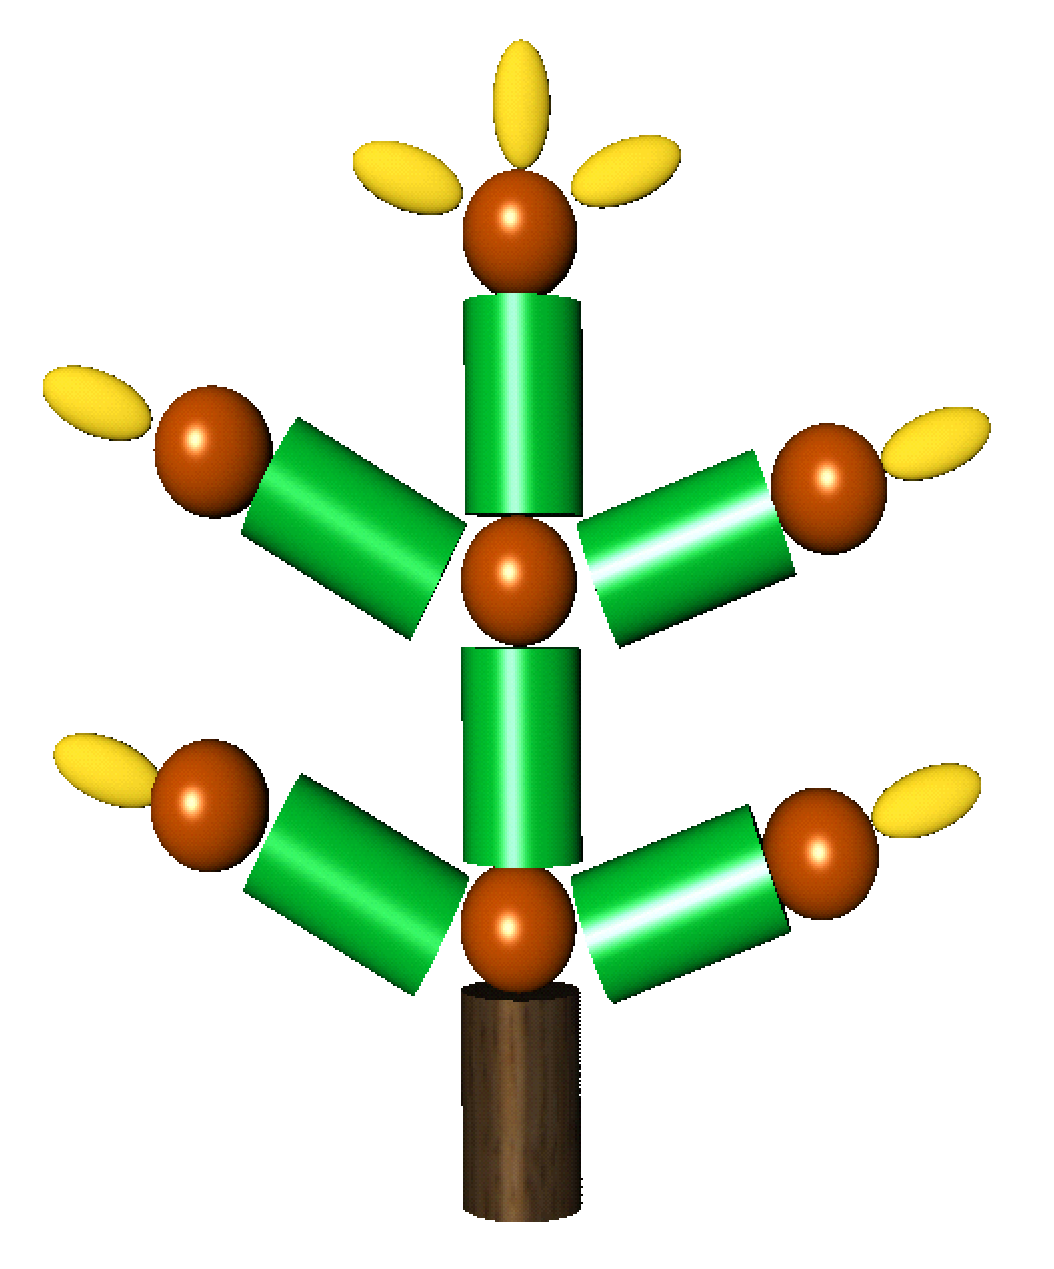
\includegraphics[scale=0.25]{cftree}
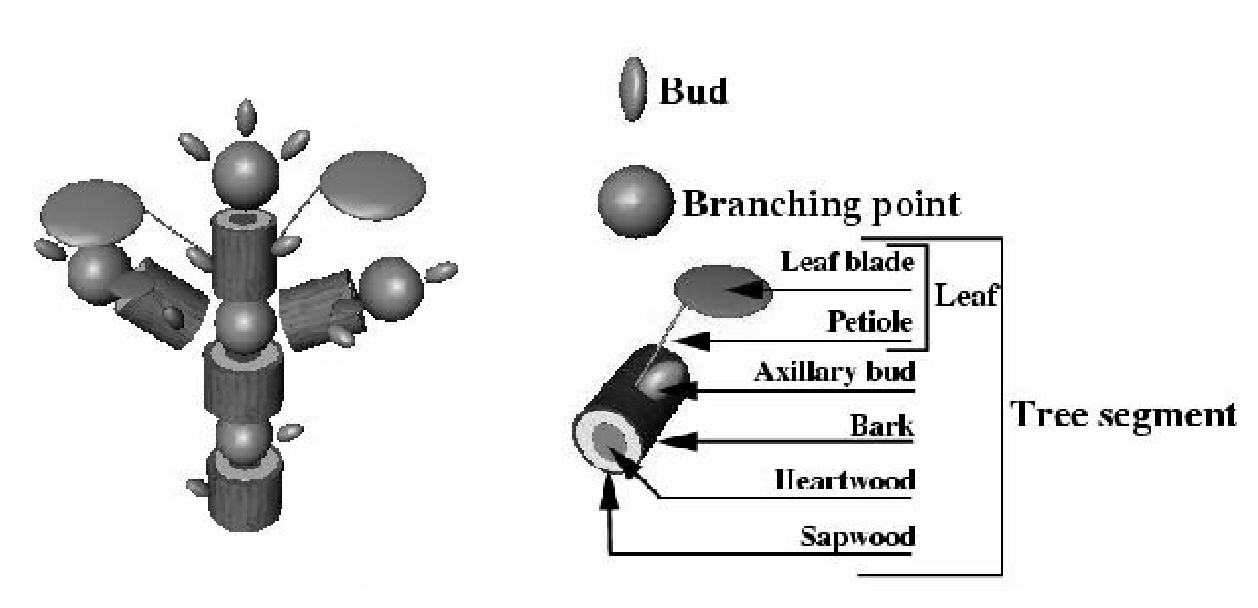
\includegraphics[scale=0.6]{hwtree}
\caption{Schematic presentation of a coniferous (left) and 
         broad-leaved tree (middle) using structural units of LIGNUM. 
         Also shown is the structure of a segment (right) 
         for broad-leaved trees}\label{fig:model} 
\end{figure}

\begin{figure}
%\makebox[\textwidth]{\framebox[10cm]{\rule{0pt}{250pt}}}
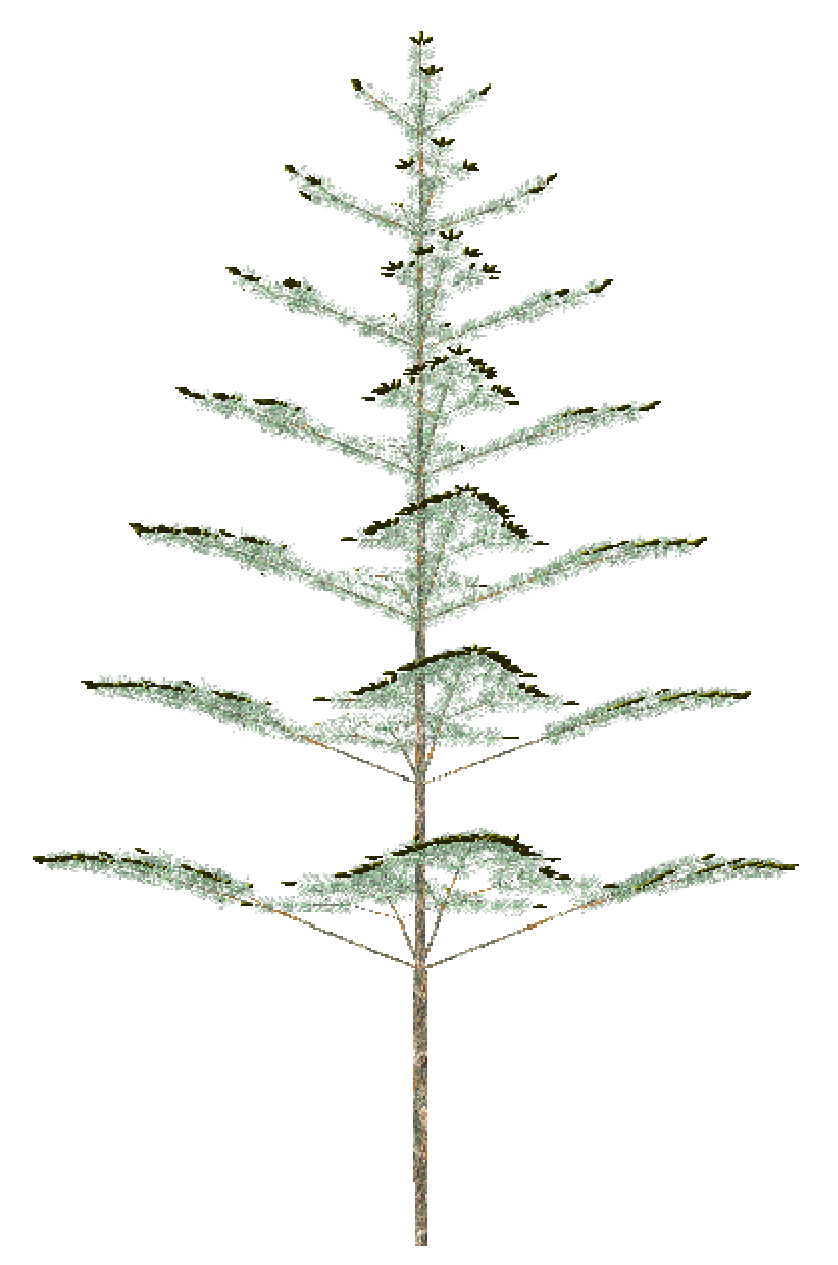
\includegraphics[scale=0.25]{pineL8}
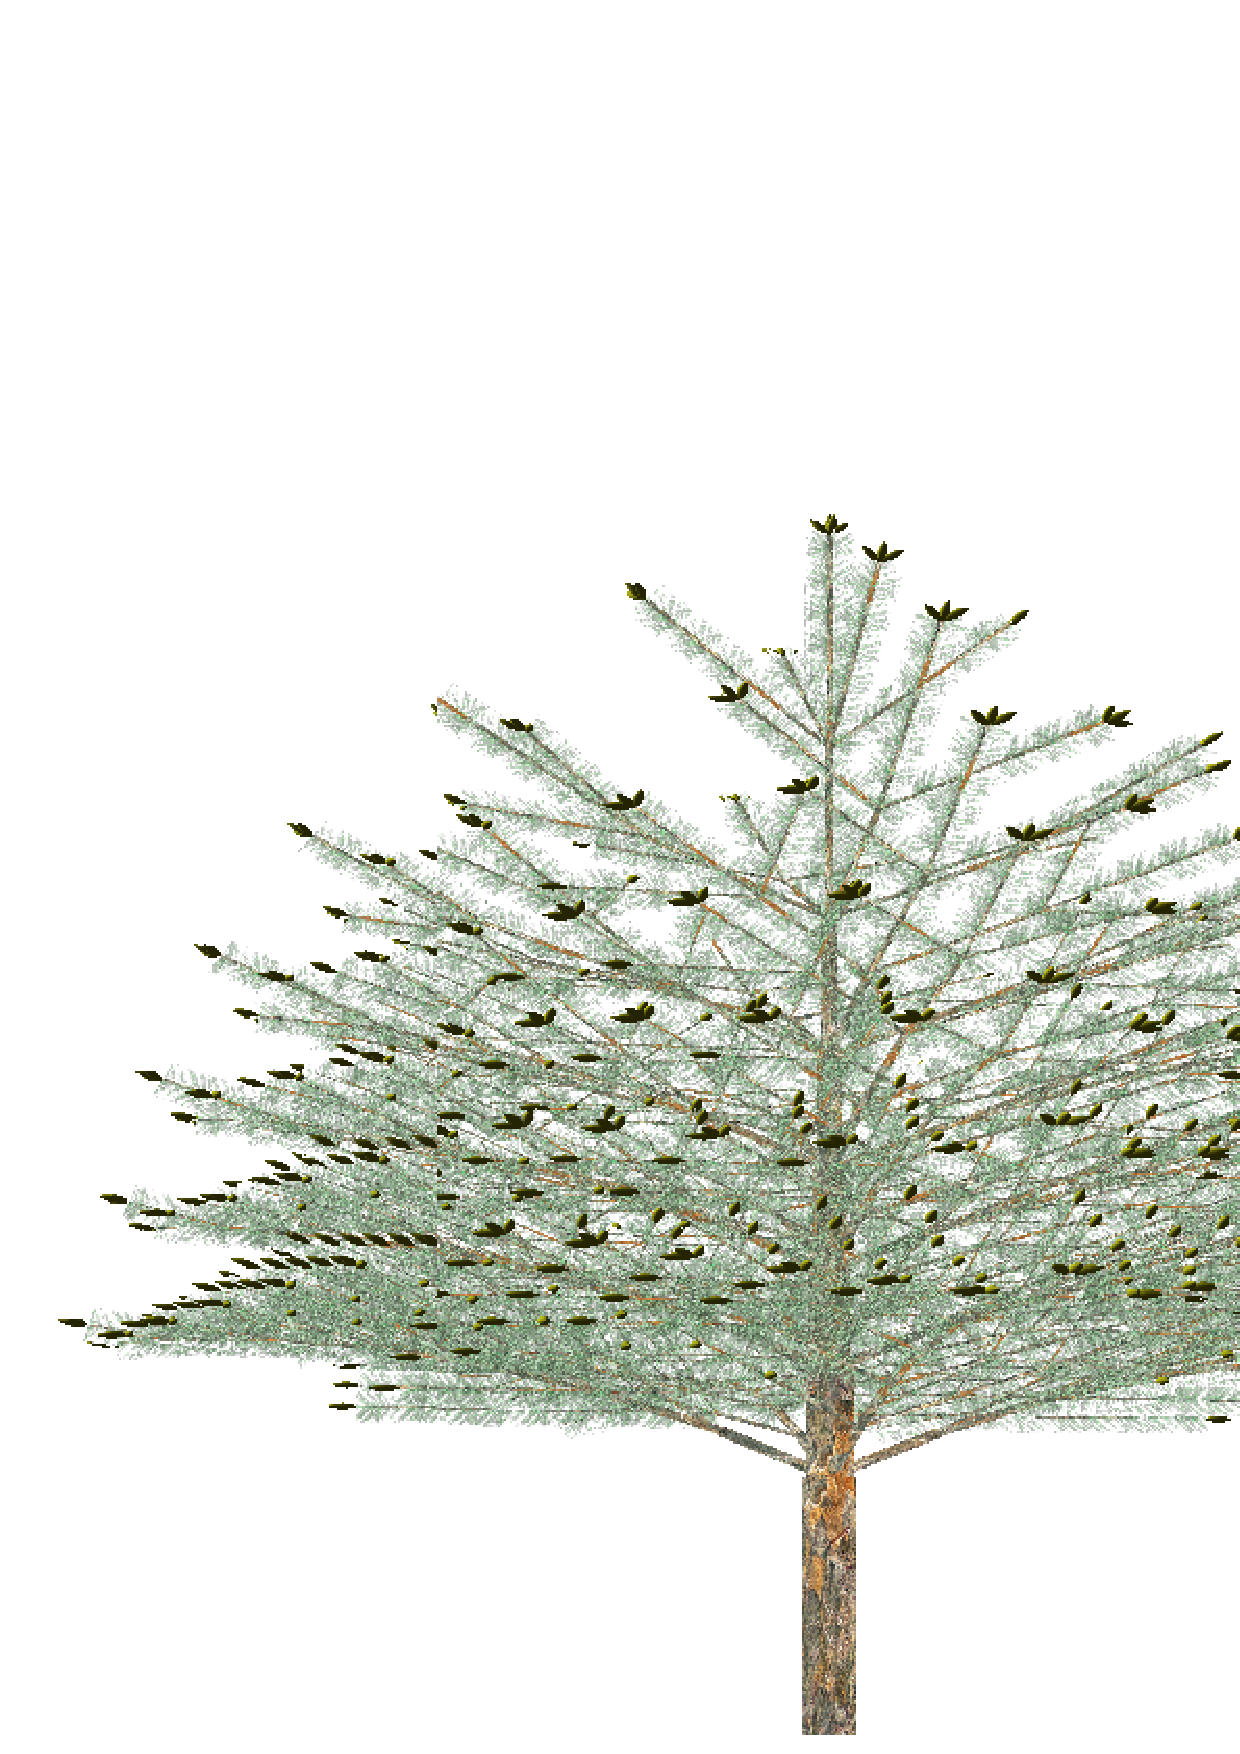
\includegraphics[scale=0.20]{pine8FEM98}
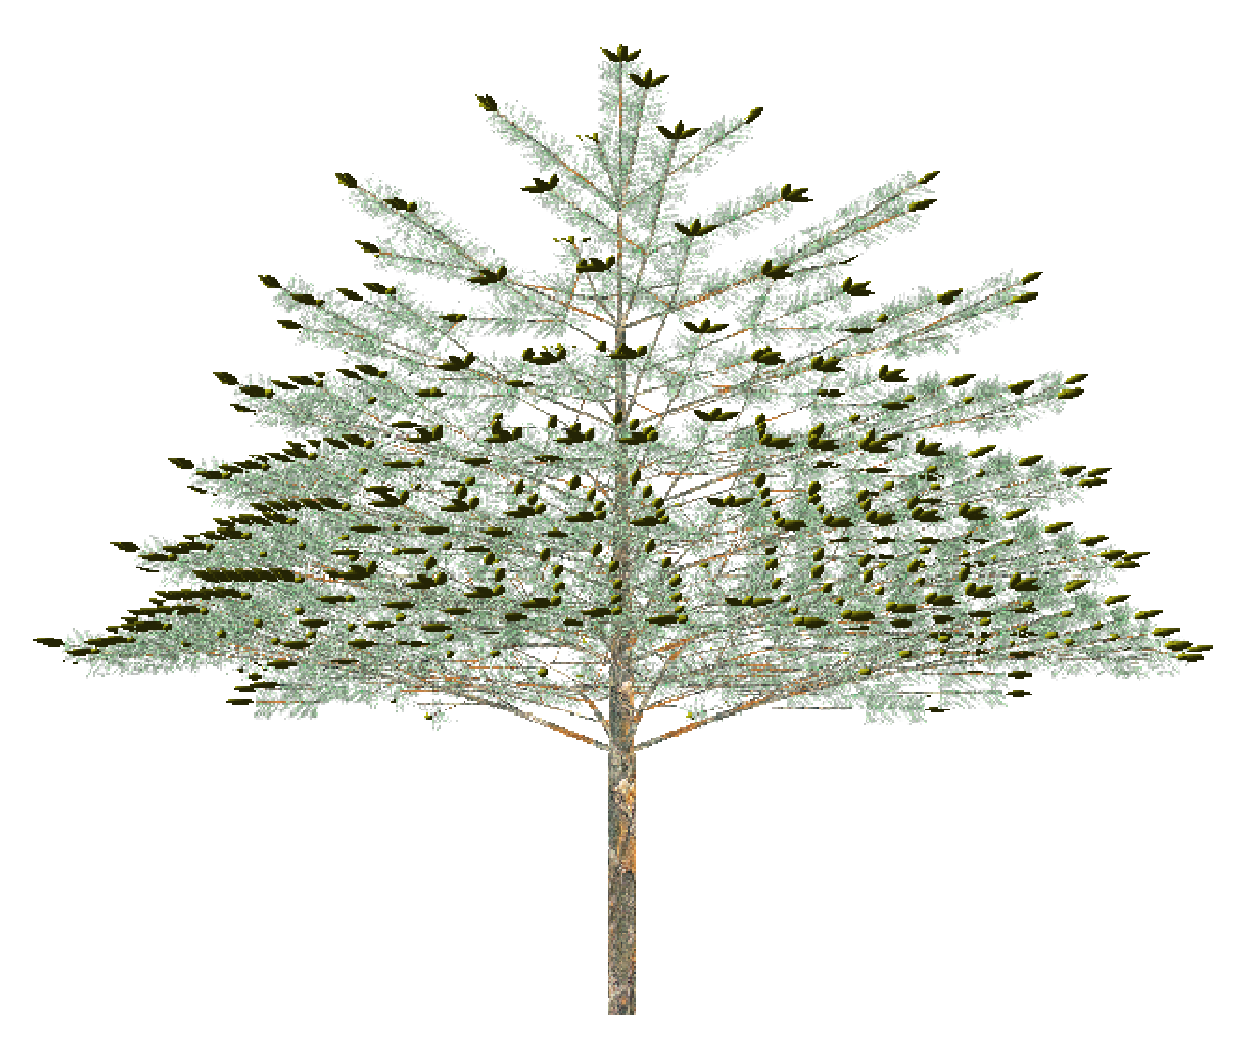
\includegraphics[scale=0.20]{pine8F1}   \caption{The   development  of
three   pines  after  eight   development  steps   when  architectural
development  takes  place  according  to  the L  program  of  Appendix
\ref{sec:L1} and  metabolic functioning is  as in \citet{perttunen:96,
perttunen:98}. We  omit some functions  of LIGNUM, e.g. the  number of
secondary buds as a function of the foliage mass of the mother segment
and  let  the L  system  determine  branching.  Leftmost:  Development
according to  the L program only;  middle and right:  interaction of L
language  and  LIGNUM  depicting  the  effect  of  foliage  mortality.
Middle: Foliage remains for 5 years.  Length = 3.5 m, diameter at base
= 10 cm.  Right: Foliage remains for 1 year.  Length = 2.7 m, diameter
at base 6 cm.}  \label{fig:pine} \end{figure}


\begin{figure}
%\makebox[\textwidth]{\framebox[10cm]{\rule{0pt}{250pt}}} 
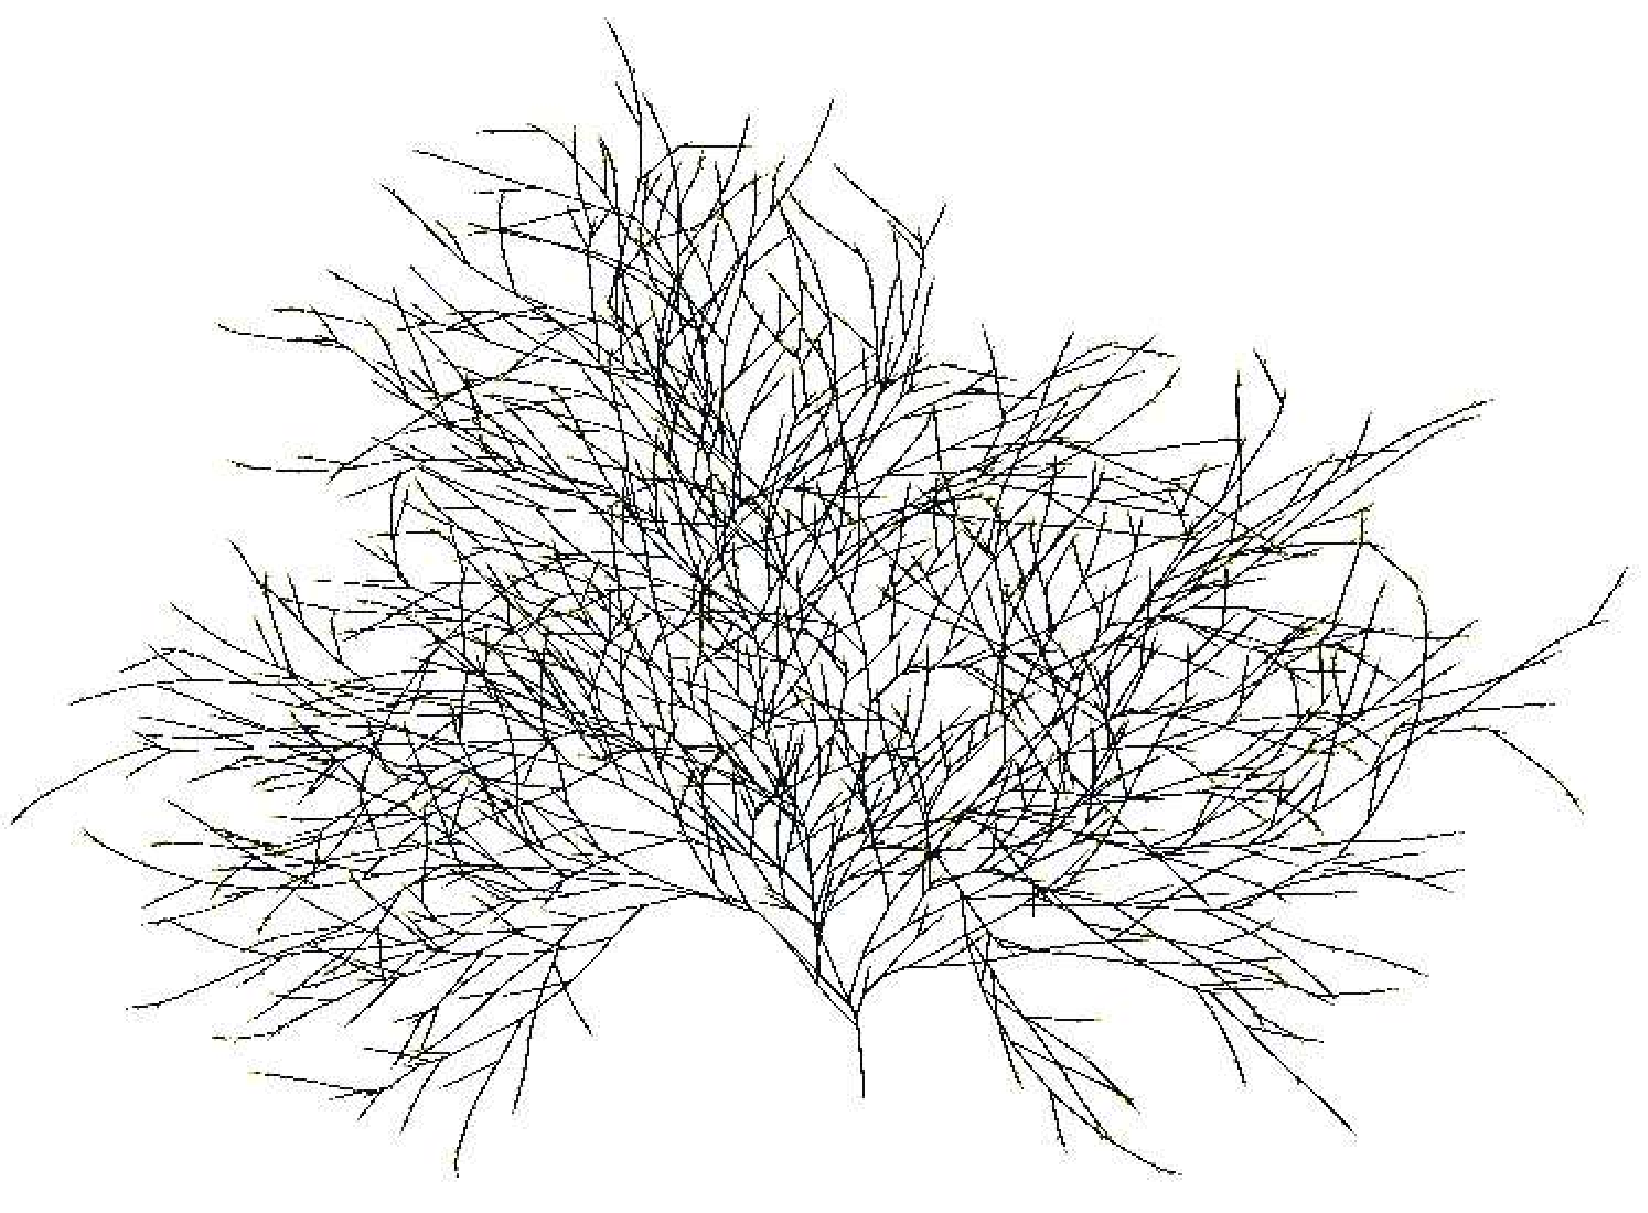
\includegraphics[scale=0.15]{auvaursi-sandpit-15-35d-30cm}
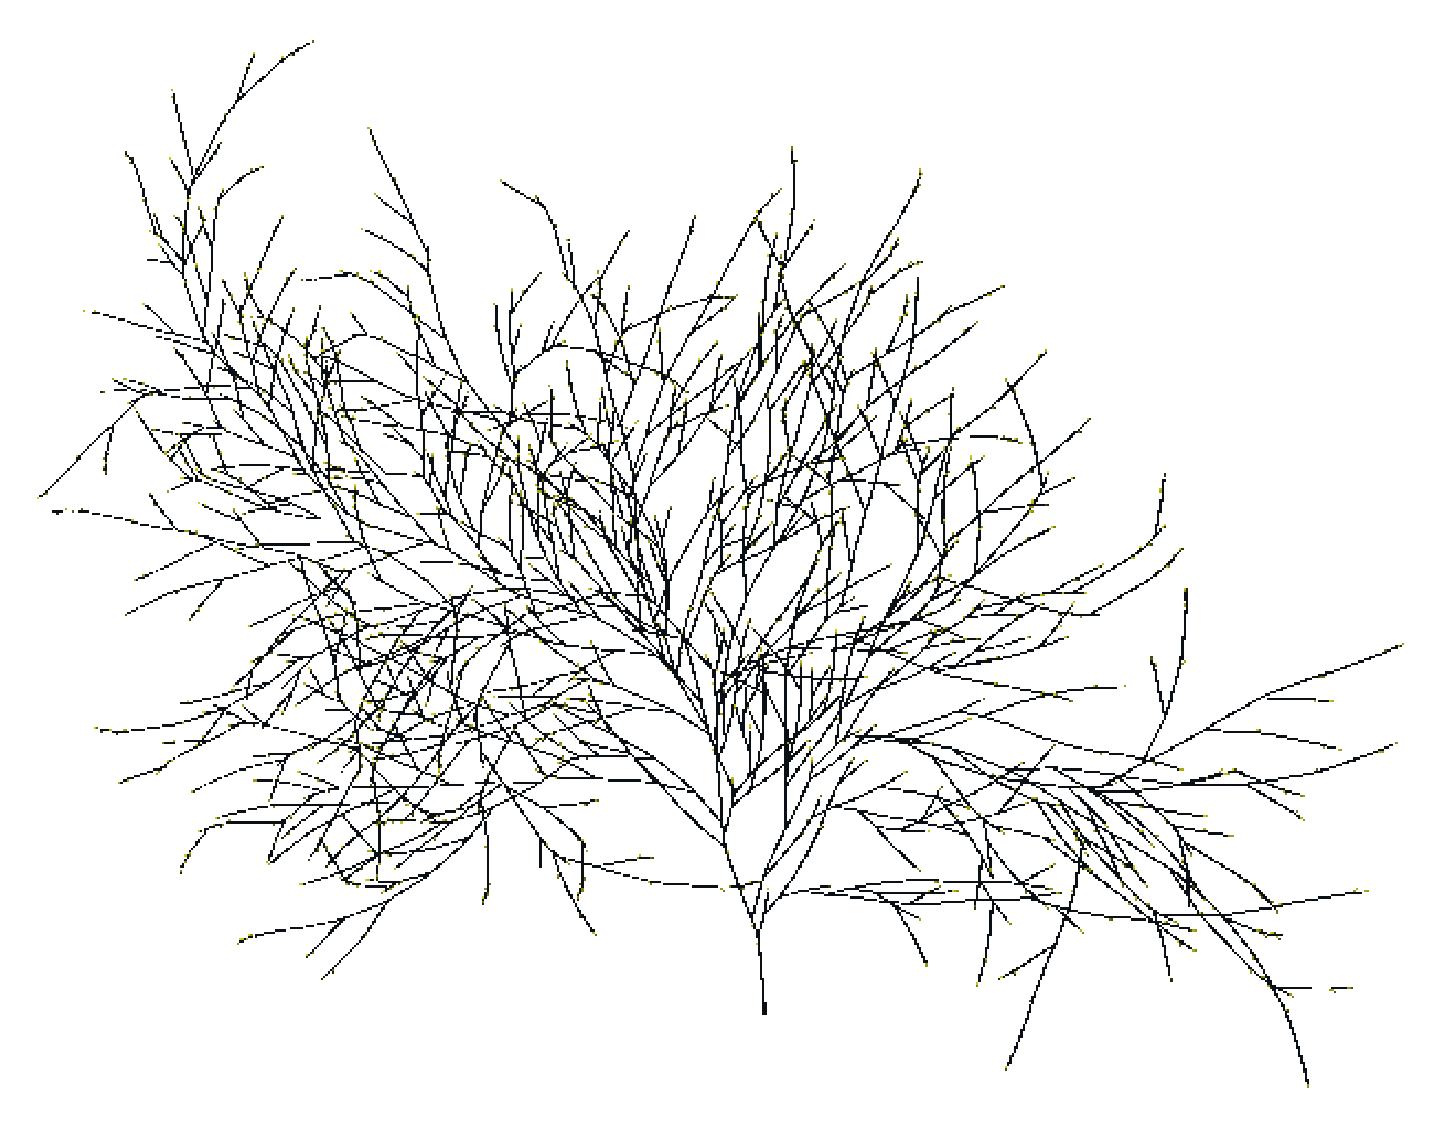
\includegraphics[scale=0.15]{auvaursi-sandpit-15-45d-30cm}
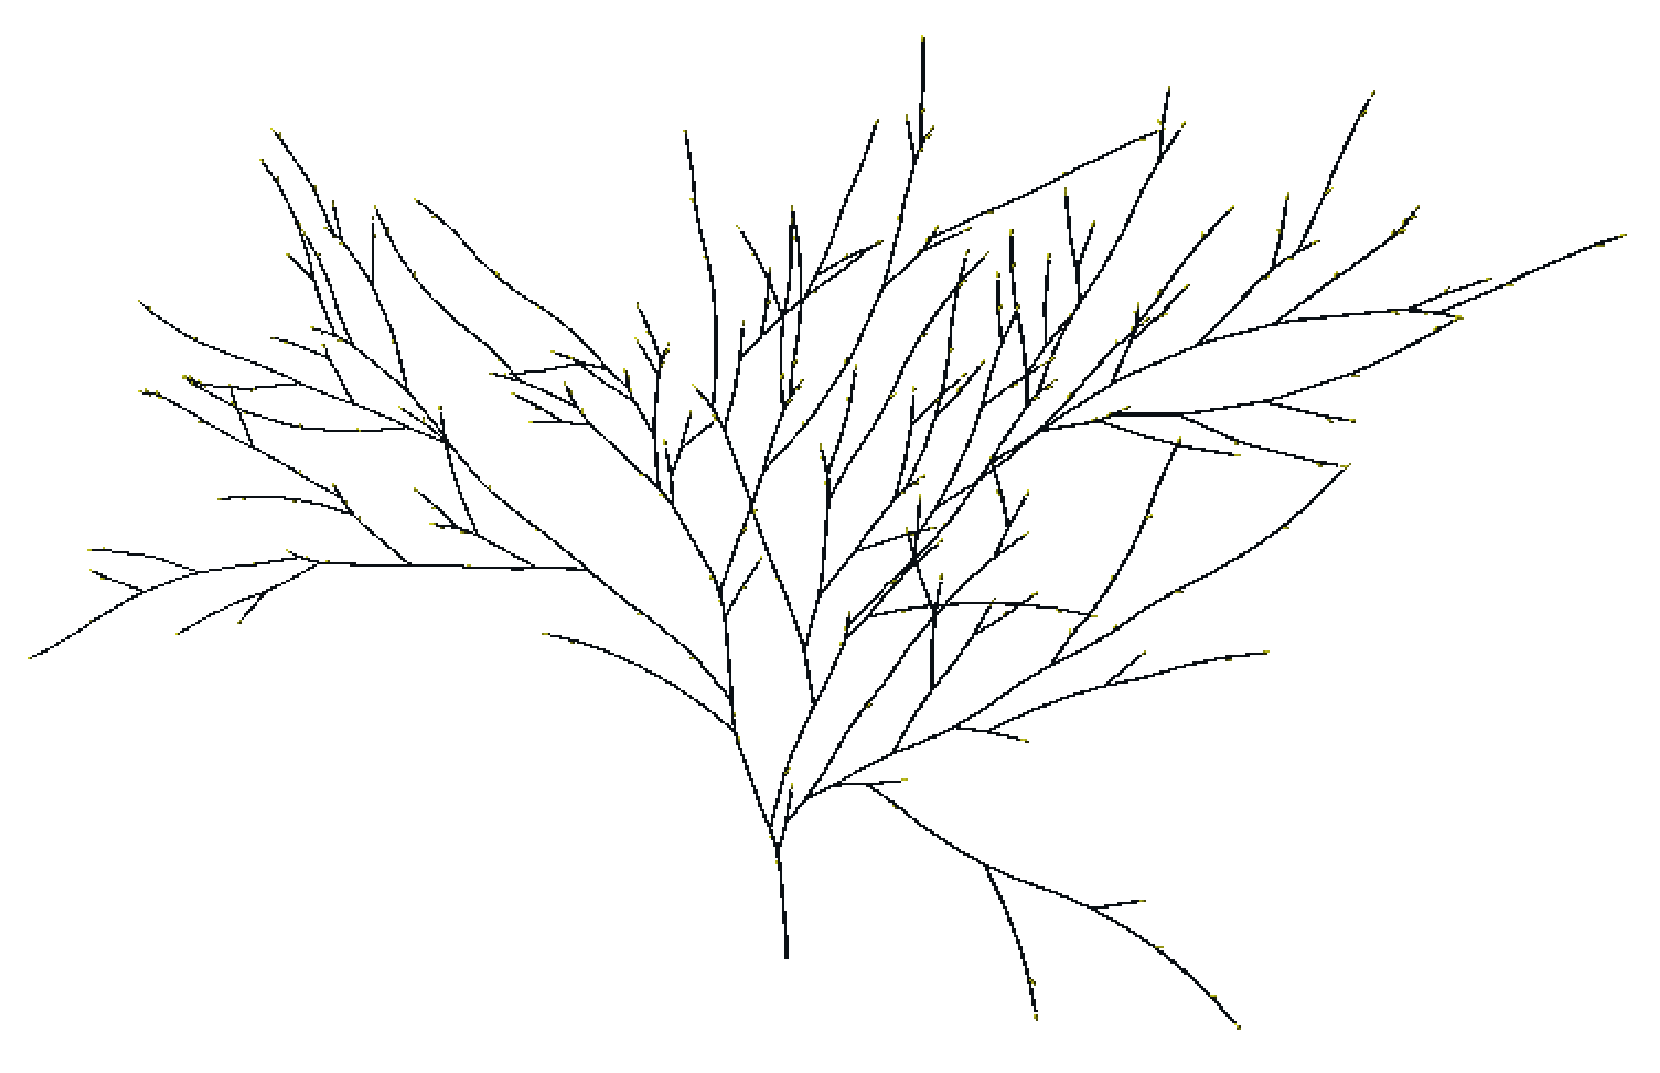
\includegraphics[scale=0.15]{auvaursi-sandpit-15-65d-30cm}    
\caption{The realization of the bearberry model by \citet{salemaa:02}
with the connection of L language program of Appendix \ref{sec:L2} and
LIGNUM.   The collision  detection is  accomplished by  LIGNUM.  Three
simulations  with 15  iterations using  different  collision detection
parameters for active buds. From  left to right: the opening angle and
the  distance  to  obstructing branch  are  $35^{\circ}/30\mathrm{cm},
45^{\circ}/30\mathrm{cm}$        and        $65^{\circ}/30\mathrm{cm}$
respectively.}\label{fig:a-uva-ursi}
\end{figure}

\pagebreak
\appendix
\section{L system mimicking pine growth}\label{sec:L1}
The L system  mimicking pine  growth starts with  one segment  and one
bud.  The main axis, ($A  = 1$),  creates one  segment and  four branches
forking off.  From then on side  branches ($A > 1$) create one segment
and  two additional  branches.  Ramification  stops after  third order
branches. Bending  of the branches  is modeled by pitching  the second
order branches ($A = 2$) down in the $Bend$ module.

%\begin{figure}[p]
%% \begin{picture}(1,1)
%% \put(0,0){\line(1,0){370}}
%% \end{picture}
\begin{verbatim}
open Pine;
const double PI = 3.1415926535897932384;
module F(double);
module B(int,double);
module Pitch(double);
module Roll(double);
module Turn(double);
module Bend(double);

Start:{produce F(0.30)SB()EB()B(1,1.0);}
B(A,l):
{
   if (A==1)
   produce F(l) SB() Pitch(PI/4.0)  B(A+1,l*0.6) EB() 
                SB() Roll(PI/2.0) Pitch(PI/4.0) B(A+1,l*0.6) EB()
                SB() Roll(PI) Pitch(PI/4.0)  B(A+1,l*0.6) EB() 
                SB() Roll(3.0*PI/2.0) Pitch(PI/4.0)  B(A+1,l*0.6) EB()
           B(A,l*0.9);
  else if (A==2)
  produce  Bend(0.3) F(l) SB() Turn(PI/4.0)  B(A+1,l*0.4) EB() 
                          SB() Turn(-PI/4.0) B(A+1,l*0.4) EB()
           Bend(-0.2)B(A,l*0.6);
  else if (A==3)
  produce F(l) SB() Turn(PI/4.0)  B(A+1,l*0.3) EB() 
               SB() Turn(-PI/4.0) B(A+1,l*0.3) EB()
          B(A,l*0.4);
  else
  produce F(l) SB() EB() B(A,l);
}
Bend(s):
{
   produce Pitch(bend);
}
close Pine;

\end{verbatim}
%% \begin{picture}(1,1)
%% \put(0,0){\line(1,0){370}}
%% \end{picture}
%\hline
%\caption{L system mimicking pine growth}\label{fig:L1}
%\end{figure}
%\pagebreak
\section{Fragmentary  L system   for  bearberry  growth}\label{sec:L2}

Fragmentary L system for  bearberry growth. The $Start$ module creates
the initial  plant.  The  $B$ module, line  15, checks  for collision.
Lines  18--40   determine  branching  and  growth.    The  pattern  of
ramification is  based on  field data and  implemented in  the uniform
random variables $r1~\mathrm{and}~r2  \in [0,1]$.  $r1$ intializes the
branching to the  left or right.  Branching and  growth depends on the
bud type,  its status and the value  of $r2$.  The counter  on line 41
eventually activates dormant buds ($s > 0$).  Bud types: D = dominant,
N  = nondominant  and  S =  subdominant.   See \citet{salemaa:02}  for
details.

%\begin{figure}[p]
%\begin{picture}(1,1)
%\put(0,0){\line(1,0){370}}
%\end{picture}
\begin{verbatim}
 1.open Bearberry;
 2.const PI = 3.1415926535897932384;
 3.module B(double type,double status,double collision); 
 4.derivation length: 15;
 5.Start:{produce F(0.1) SB() EB() B(D,0.0,0.0);}
 6.B(T,s,C):
 7.{
 8.  double g = 0.0;
 9.  double r1 = ran();
10.  double r2 = ran();
11.  if (r1 < 0.5) 
12.     g = -5*PI/180;
13.  else 
14.     g =  5*PI/180;
15.  if (C == 1.0){
16.    produce B(T,s,C);
17.  }
18.  else if (T == D && s == 0.0){
19.    if (r2 < 0.26)
20.      produce Turn(g)F(0.6)SB()Turn( 30*PI/180)B(N,2,C)EB() 
21.              Turn(g)F(0.1)SB()Turn(-30*PI/180)B(N,1,C)EB()
22.              Turn(g)F(0.1)SB()Turn( 30*PI/180)B(S,1,C)EB()
23.              Turn(g)F(0.1)SB()Turn(-30*PI/180)B(S,0,C)EB()
24.              Turn(g)F(0.1)SB()EB()B(D,0,C);
25.    else if (r2 <= 0.52)
26.      produce Turn(g)F(0.6)SB()Turn(-30*PI/180)B(N,2,C)EB() 
27.              Turn(g)F(0.1)SB()Turn( 30*PI/180)B(N,1,C)EB()
26.              Turn(g)F(0.1)SB()Turn(-30*PI/180)B(S,1,C)EB()
28.              Turn(g)F(0.1)SB()Turn( 30*PI/180)B(S,0,C)EB()
29.              Turn(g)F(0.1)SB()EB()B(D,0,C);
30       ......................................................
32.  } 
33.  else if (T == S && s == 0.0){
33.    if (r2 < 0.037)
34.      produce Turn(g)F(0.48)SB()Turn(-30*PI/180)B(S,1,C)EB()
35.              Turn(g)F(0.08)SB()EB()B(S,0,C);
36.       ......................................................
37.  }
38.  else if (T == N && s == 0.0){
39.       ......................................................
40.  else{
41.    produce B(T,max(s-1,0),C);
42.  }
43.}
44.close Bearberry;
\end{verbatim}
%\begin{picture}(1,1)
%\put(0,0){\line(1,0){370}}
%\end{picture}
%\caption{)
%\end{figure}





% Parenthetical: \citep{Bai92} produces (Bailyn 1992).
% Textual: \citet{Bai95} produces Bailyn et al. (1995).
% An affix and part of a reference:
%   \citep[e.g.][Ch. 2]{Bar76}
%   produces (e.g. Barnes et al. 1976, Ch. 2).

%\begin{thebibliography}{}

% \bibitem[Names(Year)]{label} or \bibitem[Names(Year)Long names]{label}.
% (\harvarditem{Name}{Year}{label} is also supported.)
% Text of bibliographic item

%\bibitem[]{}

%\end{thebibliography}

\end{document}







